% ======================================================================
%  Proposed Clustering-MoE (ClusterMoE) Architecture -- IEEE style figure
%  Compile with pdflatex / Overleaf.  Standalone -> crops to the figure.
%  In an IEEE paper, drop the body inside \begin{figure*}...\end{figure*}.
% ======================================================================
\documentclass[border=4pt,tikz]{standalone}
\usepackage{tikz}
\usepackage{amsmath}
\usepackage{amssymb}
\usepackage[T1]{fontenc}
\usepackage{helvet}
\renewcommand{\familydefault}{\sfdefault}   % IEEE figures: sans-serif labels
\usetikzlibrary{arrows.meta,positioning,fit,backgrounds,calc,shapes.geometric}

\begin{document}
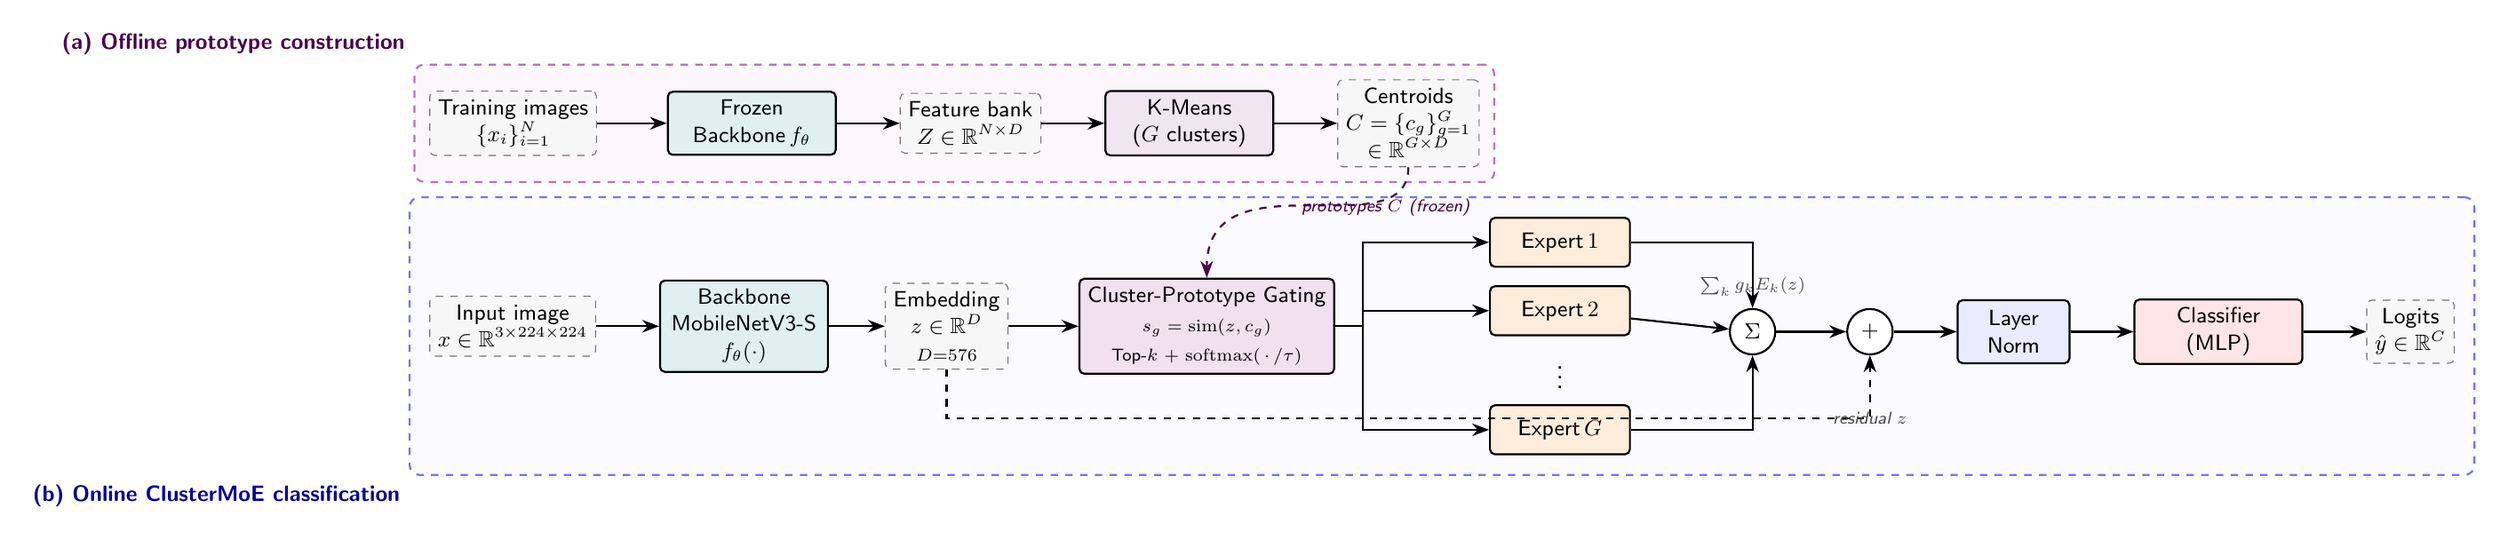
\begin{tikzpicture}[
    font=\small,
    >={Stealth[length=2.4mm]},
    block/.style   ={rectangle, rounded corners=2pt, draw=black, thick,
                     minimum width=24mm, minimum height=9mm, align=center,
                     fill=blue!6},
    bb/.style      ={block, fill=teal!12},
    expert/.style  ={block, minimum width=20mm, minimum height=7mm,
                     fill=orange!14},
    gate/.style    ={block, fill=violet!12, minimum width=30mm},
    op/.style      ={circle, draw=black, thick, minimum size=6.5mm,
                     inner sep=0pt, fill=white},
    cls/.style     ={block, fill=red!10},
    data/.style    ={rectangle, draw=black!55, dashed, rounded corners=2pt,
                     minimum height=8mm, align=center, fill=gray!6},
    flow/.style    ={->, thick},
    lbl/.style     ={font=\scriptsize\itshape, text=black!70},
]

% ----------------------------------------------------------------------
%  (A) OFFLINE STAGE : feature extraction + K-Means prototypes
% ----------------------------------------------------------------------
\node[data]  (trainset) {Training images\\$\{x_i\}_{i=1}^{N}$};
\node[bb, right=10mm of trainset] (bbfrozen) {Frozen\\Backbone\,$f_\theta$};
\node[data, right=9mm of bbfrozen] (feats) {Feature bank\\$Z\in\mathbb{R}^{N\times D}$};
\node[block, right=9mm of feats, fill=violet!10] (kmeans)
        {K-Means\\($G$ clusters)};
\node[data, right=9mm of kmeans] (cents)
        {Centroids\\$C=\{c_g\}_{g=1}^{G}$\\$\in\mathbb{R}^{G\times D}$};

\draw[flow] (trainset) -- (bbfrozen);
\draw[flow] (bbfrozen) -- (feats);
\draw[flow] (feats)    -- (kmeans);
\draw[flow] (kmeans)   -- (cents);

\begin{scope}[on background layer]
  \node[draw=violet!55, dashed, thick, rounded corners=4pt, fill=violet!3,
        fit=(trainset)(bbfrozen)(feats)(kmeans)(cents),
        inner sep=6pt, label={[violet!60!black,font=\small\bfseries]north west:%
        (a) Offline prototype construction}] (offlinebox) {};
\end{scope}

% ----------------------------------------------------------------------
%  (B) ONLINE STAGE : ClusterMoE inference path  (placed below)
% ----------------------------------------------------------------------
\node[data, below=20mm of trainset.south west, anchor=north west]
        (img) {Input image\\$x\in\mathbb{R}^{3\times224\times224}$};
\node[bb, right=9mm of img] (backbone)
        {Backbone\\MobileNetV3-S\\$f_\theta(\cdot)$};
\node[data, right=8mm of backbone] (emb)
        {Embedding\\$z\in\mathbb{R}^{D}$\\\scriptsize$D{=}576$};

% --- Gating router ---
\node[gate, right=10mm of emb] (gating)
        {Cluster-Prototype Gating\\[1pt]
         \scriptsize$s_g=\mathrm{sim}(z,c_g)$\\[1pt]
         \scriptsize Top-$k$ $+\ \mathrm{softmax}(\,\cdot\,/\tau)$};

% --- Experts stack ---
\node[expert, right=22mm of gating, yshift=12mm] (e1) {Expert\,$1$};
\node[expert, below=2.5mm of e1]                 (e2) {Expert\,$2$};
\node[font=\large, below=1mm of e2]              (edots) {$\vdots$};
\node[expert, below=1mm of edots]                (eG) {Expert\,$G$};

% --- combine / residual / norm / classifier ---
\node[op, right=14mm of e2, yshift=-3mm] (sum) {$\Sigma$};
\node[op, right=10mm of sum]            (res) {$+$};
\node[block, right=9mm of res, fill=blue!8, minimum width=16mm] (norm)
        {Layer\\Norm};
\node[cls, right=9mm of norm] (clsf)
        {Classifier\\(MLP)};
\node[data, right=9mm of clsf] (logits) {Logits\\$\hat{y}\in\mathbb{R}^{C}$};

% --- edges of online path ---
\draw[flow] (img)      -- (backbone);
\draw[flow] (backbone) -- (emb);
\draw[flow] (emb)      -- (gating);

% emb feeds experts (fan-out) and the residual branch
\coordinate (embsplit) at ($(emb.east)+(4mm,0)$);
\draw[flow] (gating.east) -- ++(4mm,0) |- (e1.west);
\draw[flow] (gating.east) -- ++(4mm,0) |- (e2.west);
\draw[flow] (gating.east) -- ++(4mm,0) |- (eG.west);

% experts -> weighted sum
\draw[flow] (e1) -| (sum);
\draw[flow] (e2) -- (sum);
\draw[flow] (eG) -| (sum);

% gating weights into the sum (g_k)
\node[lbl, above=0.5mm of sum] {$\sum_k g_k E_k(z)$};

\draw[flow] (sum)  -- (res);
\draw[flow] (norm) -- (clsf);
\draw[flow] (res)  -- (norm);
\draw[flow] (clsf) -- (logits);

% residual skip connection: z  ->  (+)
\draw[flow, dashed] (emb.south) |- ($(res.south)+(0,-9mm)$) -- (res.south)
      node[lbl, pos=0.25, below] {residual $z$};

% centroids feed the gating (cross-stage link)
\draw[flow, violet!60!black, thick, dashed]
      (cents.south) .. controls +(0,-12mm) and +(0,18mm) .. (gating.north)
      node[lbl, text=violet!55!black, pos=0.55, right] {prototypes $C$ (frozen)};

\begin{scope}[on background layer]
  \node[draw=blue!55, dashed, thick, rounded corners=4pt, fill=blue!2,
        fit=(img)(backbone)(emb)(gating)(e1)(eG)(sum)(res)(norm)(clsf)(logits),
        inner sep=8pt,
        label={[blue!60!black,font=\small\bfseries]south west:%
        (b) Online ClusterMoE classification}] (onlinebox) {};
\end{scope}

\end{tikzpicture}
\end{document}
